
\section{UML Models}

\subsection{Use Case Diagram}

With the Use Case Diagram are highlighted the main function of our
system and the interaction between ACTORS and the related Use Case.
\begin{center}
\begin{figure}[H]
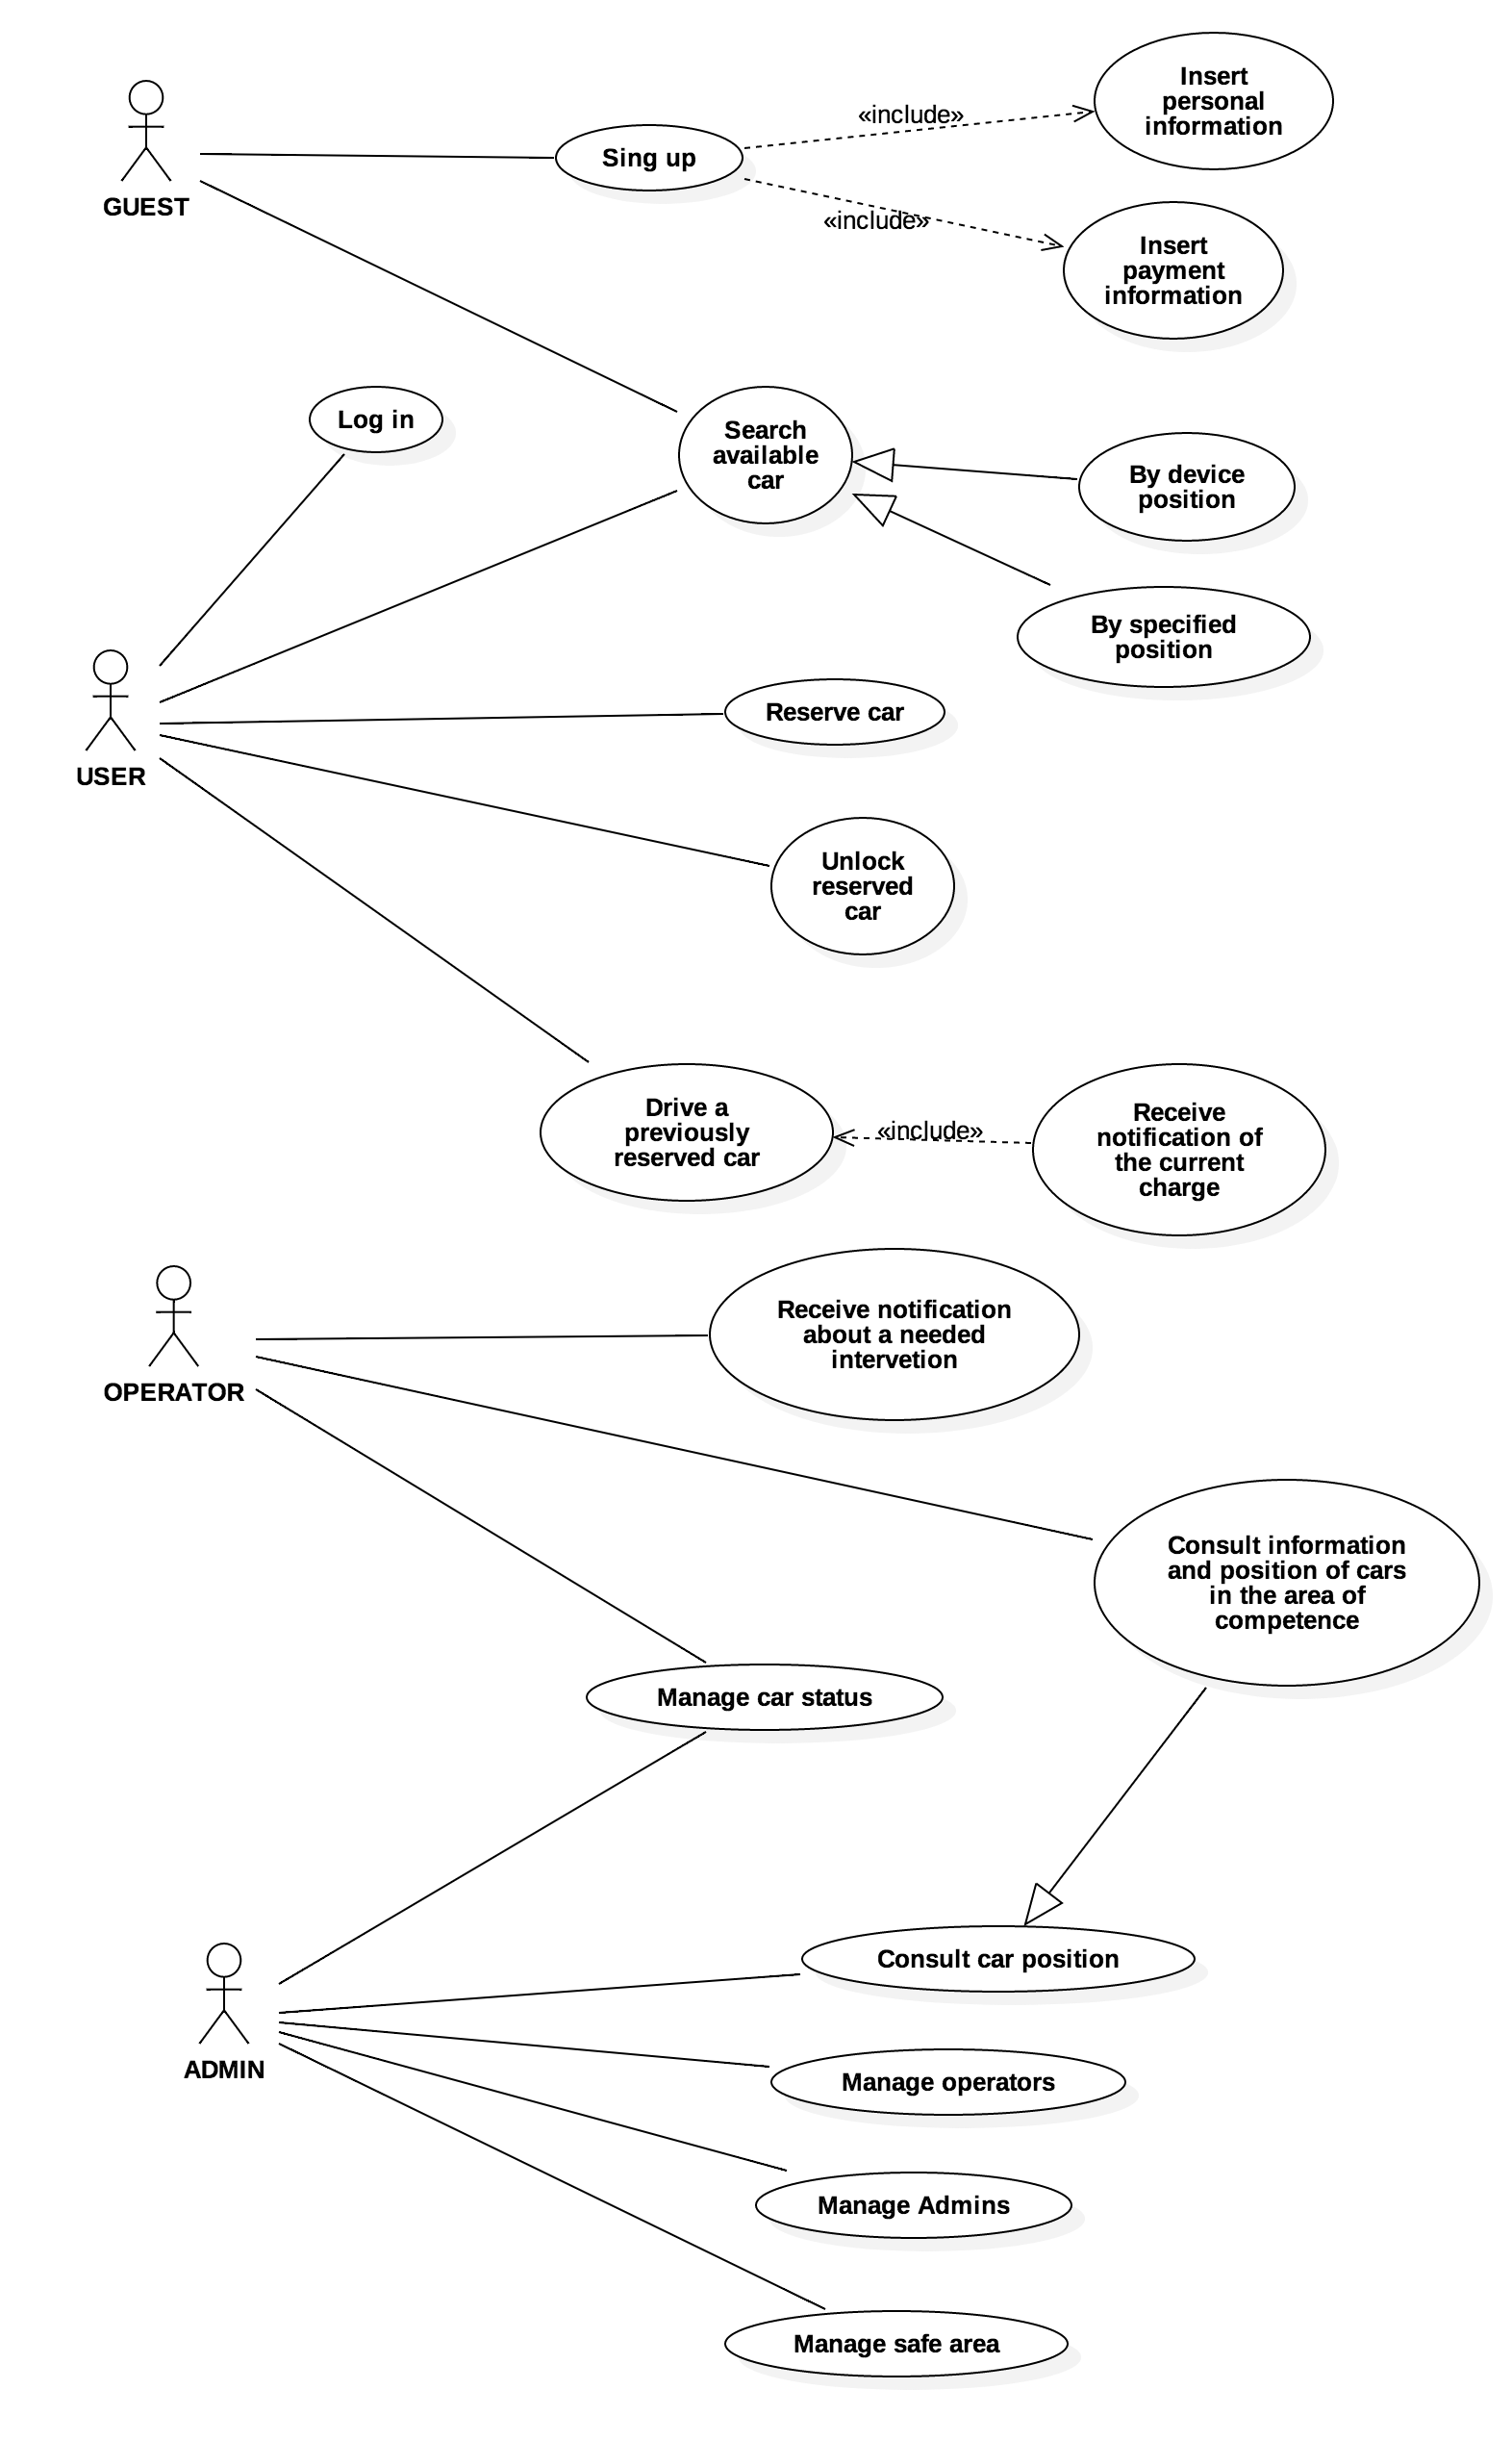
\includegraphics[clip,scale=0.15]{UML/png/Model__UseCaseDiagram1_1}

\caption{Use Case Diagram}

\end{figure}
\par\end{center}

\subsection{Sequence Diagram}

With Sequence Diagram are highlighted the main function of the system
and the High-Level sequence of actions that focuses on the way in
which happens the interaction between ACTORS and system.

\subsubsection{Registration}
\begin{flushleft}
\begin{tabular}{|c|>{\raggedright}p{10cm}|}
\hline 
$\boldsymbol{\mathbf{Name}}$ & Registration\tabularnewline
\hline 
$\mathbf{Actors}$ & Guest\tabularnewline
\hline 
$\mathbf{Goal}$ & All\tabularnewline
\hline 
$\mathbf{EntryConditions}$ & Guest isn't already registered to the application.\tabularnewline
\hline 
$\mathbf{EventFlow}$ & \begin{enumerate}
\item Guest opens the app.
\item Guest click on Sign Up button.
\item Guest fills in all mandatory fields like payment informations, his
vital statistics etc.
\item Form is sent to the server that saves all data in the DB.
\item Email with registration confirmation is sent by the server to the
email address provided in the form.
\end{enumerate}
\tabularnewline
\hline 
$\mathbf{Output}$ $\mathbf{Condition}$ & GUEST ends registration procedure and become a USER. Now he/she can
login and use all functionalities offeredby the system.\tabularnewline
\hline 
$\mathbf{Exception}$ & \begin{enumerate}
\item Payment informations are not valid.
\item Driving License in not valid.
\item Username is already used by another user.
\item One or more mandatory fields of the form are not valid.
\end{enumerate}
In all this case the visitor is alert and the app explains the problem.
Then the app goes back to point 3 of Event Flow.\tabularnewline
\hline 
\end{tabular}\\
\par\end{flushleft}

\begin{center}
\begin{figure}[H]
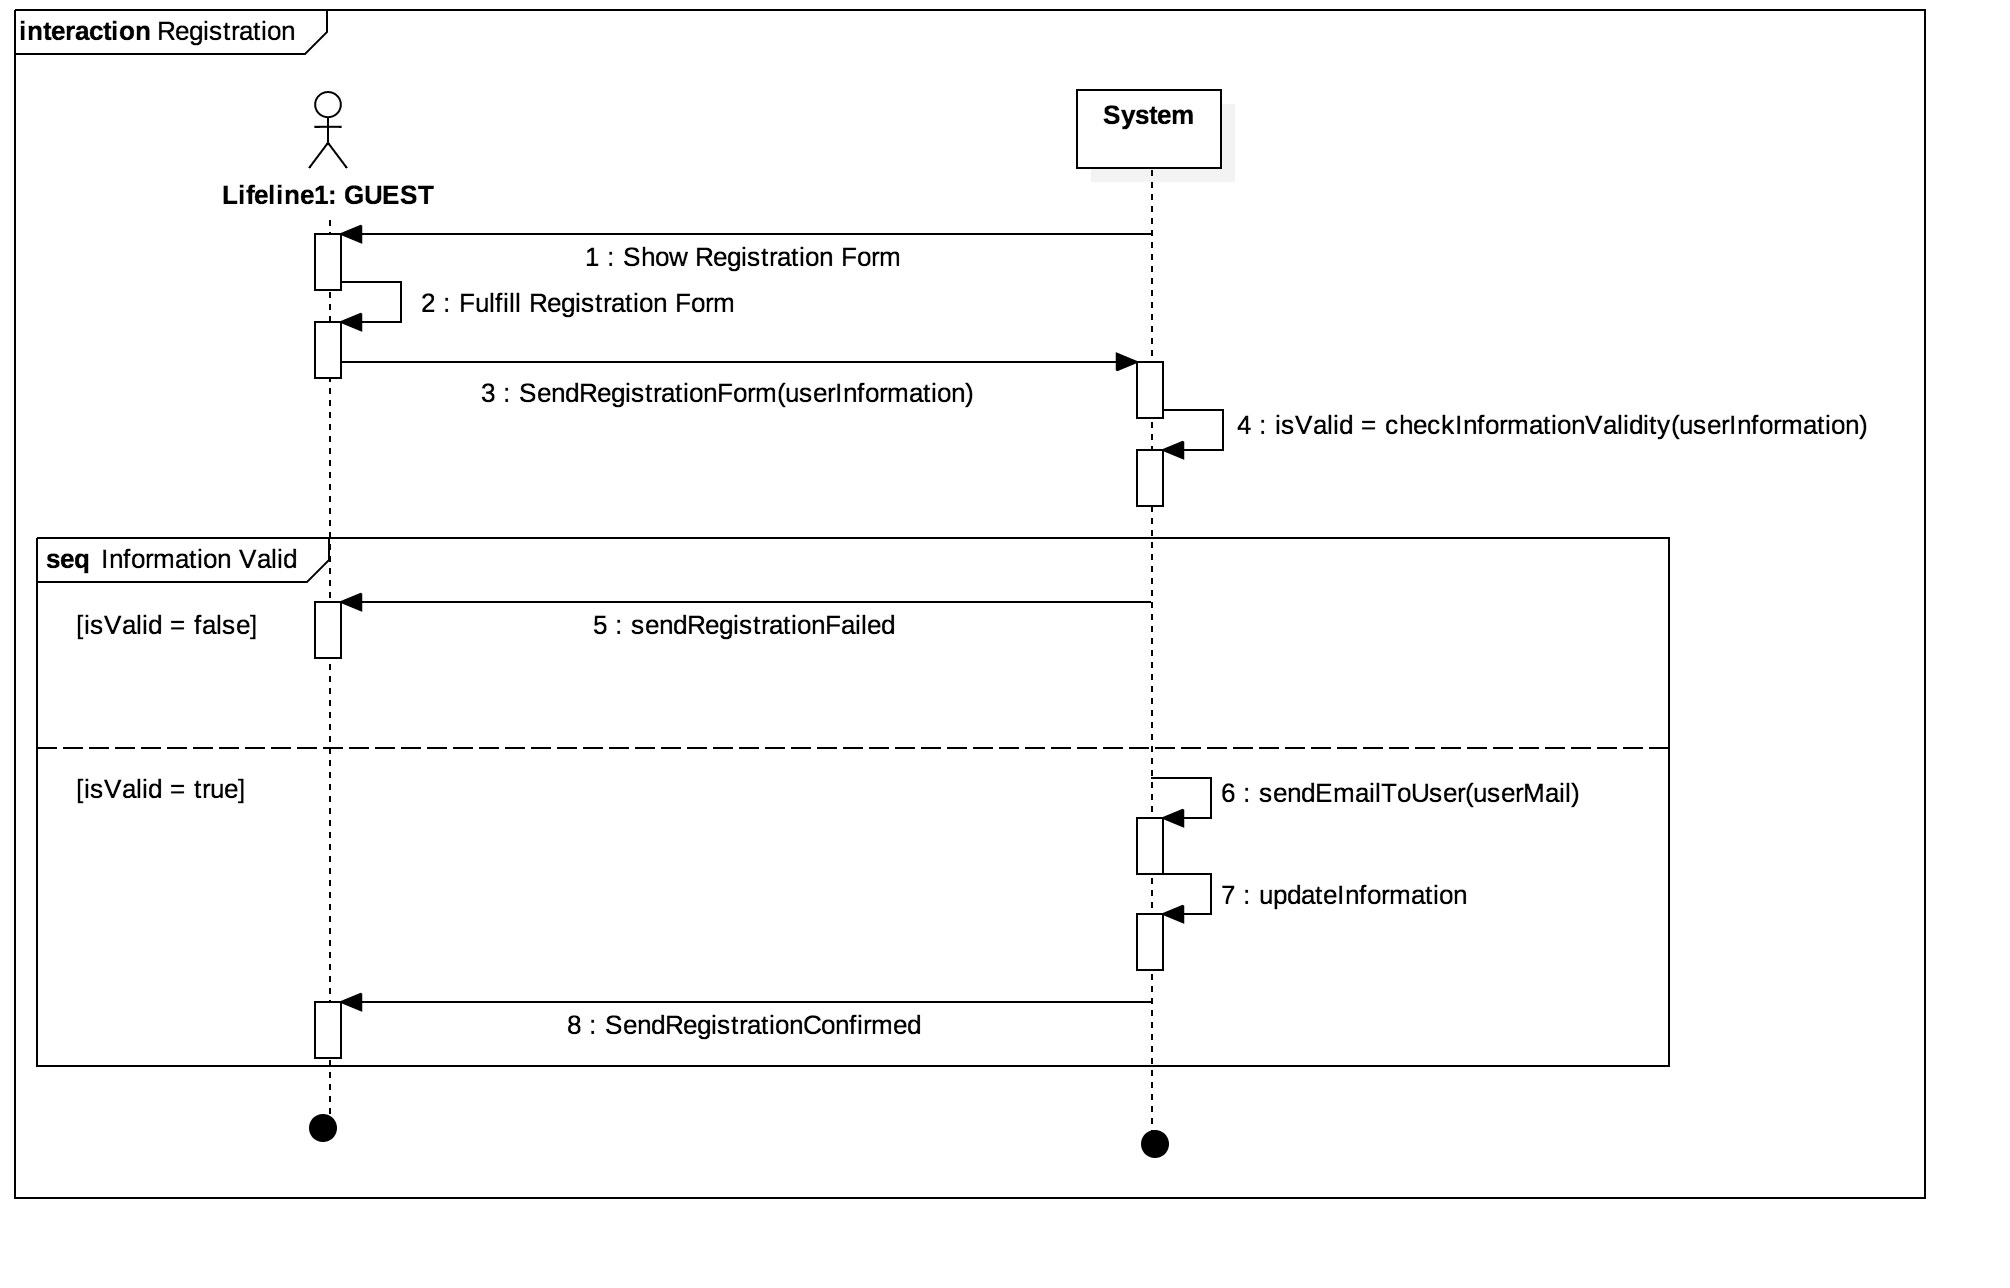
\includegraphics[scale=0.3]{UML/png/Collaboration6__Interaction1__Registration_8}

\caption{Registration}

\end{figure}
\\
\\
\par\end{center}

\subsubsection{Login}

\begin{tabular}{|c|>{\raggedright}p{10cm}|}
\hline 
$\boldsymbol{\mathbf{Name}}$ & Login\tabularnewline
\hline 
$\mathbf{Actors}$ & USER\tabularnewline
\hline 
$\mathbf{Goal}$ & All\tabularnewline
\hline 
$\mathbf{EntryConditions}$ & USER is registered into the system\tabularnewline
\hline 
$\mathbf{EventFlow}$ & \begin{enumerate}
\item User opens the app.
\item App shows login page.
\item User inserts his email and his password.
\item Email and password are sent to server in a secure way.
\item Server verifies user's credentials and confirms login.
\end{enumerate}
\tabularnewline
\hline 
$\mathbf{OutputCondition}$ & User can use the app, reserve cars and consult his profile.\tabularnewline
\hline 
$\mathbf{Exception}$ & \begin{enumerate}
\item User's credentials are incorrect.
\item User is banned to the system (due to an incorrect behaviour).
\end{enumerate}
In the first case the user is notified that his/her credentials are
incorrect. \\
In the second case the user is notified that he can't use the service
because of his behaviour. \tabularnewline
\hline 
\end{tabular}\\
\\

\begin{center}
\begin{figure}[H]
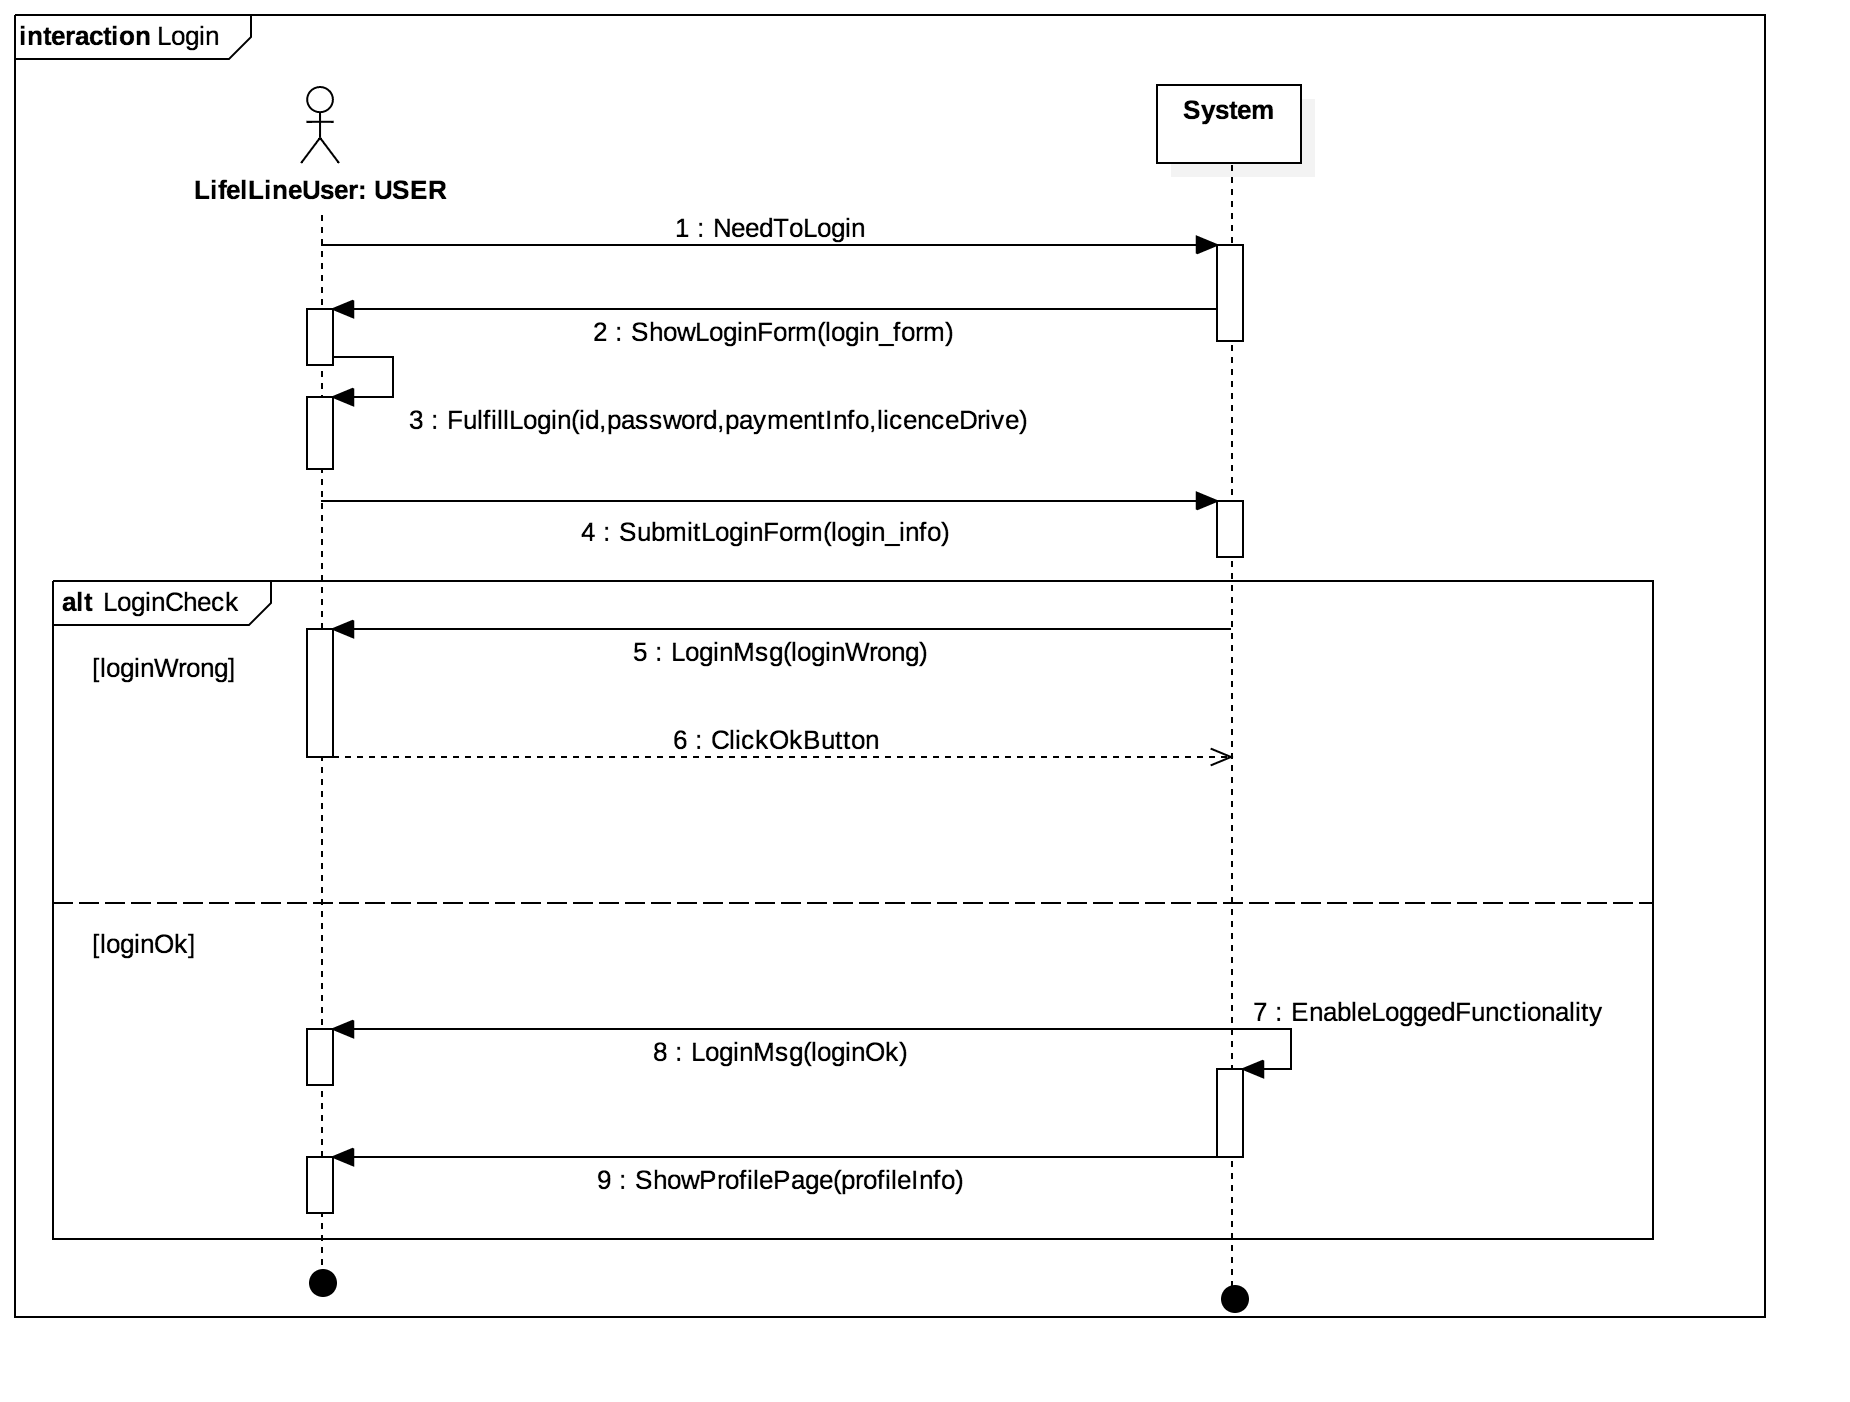
\includegraphics[scale=0.2]{UML/png/Collaboration1__Interaction1__Login_2}

\caption{Login}

\end{figure}
\par\end{center}

\subsubsection{Car Reservation}

\begin{tabular}{|c|>{\raggedright}p{10cm}|}
\hline 
$\boldsymbol{\mathbf{Name}}$ & Car Reservation\tabularnewline
\hline 
$\mathbf{Actors}$ & USER\tabularnewline
\hline 
$\mathbf{Goal}$ & {[}G1.1{]}\tabularnewline
\hline 
$\mathbf{EntryConditions}$ & USER is registered into the system and has already logged in.\tabularnewline
\hline 
$\mathbf{EventFlow}$ & \begin{enumerate}
\item USER selects a car.
\item User fills the reservation form with the reservation hour.
\item Form is sent to the server.
\item Server verifyies the form and the validity of reservation.
\item Server updates his informations with the new reservation.
\item App confirms reservation to the user.
\item App adds to current user's reservation the actual reservation.
\end{enumerate}
\tabularnewline
\hline 
$\mathbf{OutputCondition}$ & User has reserved a car and he can use it.\tabularnewline
\hline 
$\mathbf{Exception}$ & \begin{enumerate}
\item Car is already reserved by another user.
\item User has already reserved another car.
\end{enumerate}
In the first case app notifies the user that he needs to select another
car in order to make his reservation. App returns to point 1 of Event
Flow.

In the second case appp notifies user that he has already reserved
another car and that he can't reserve more than one car at the same
time.\tabularnewline
\hline 
\end{tabular}\\
\\

\begin{center}
\begin{figure}[H]
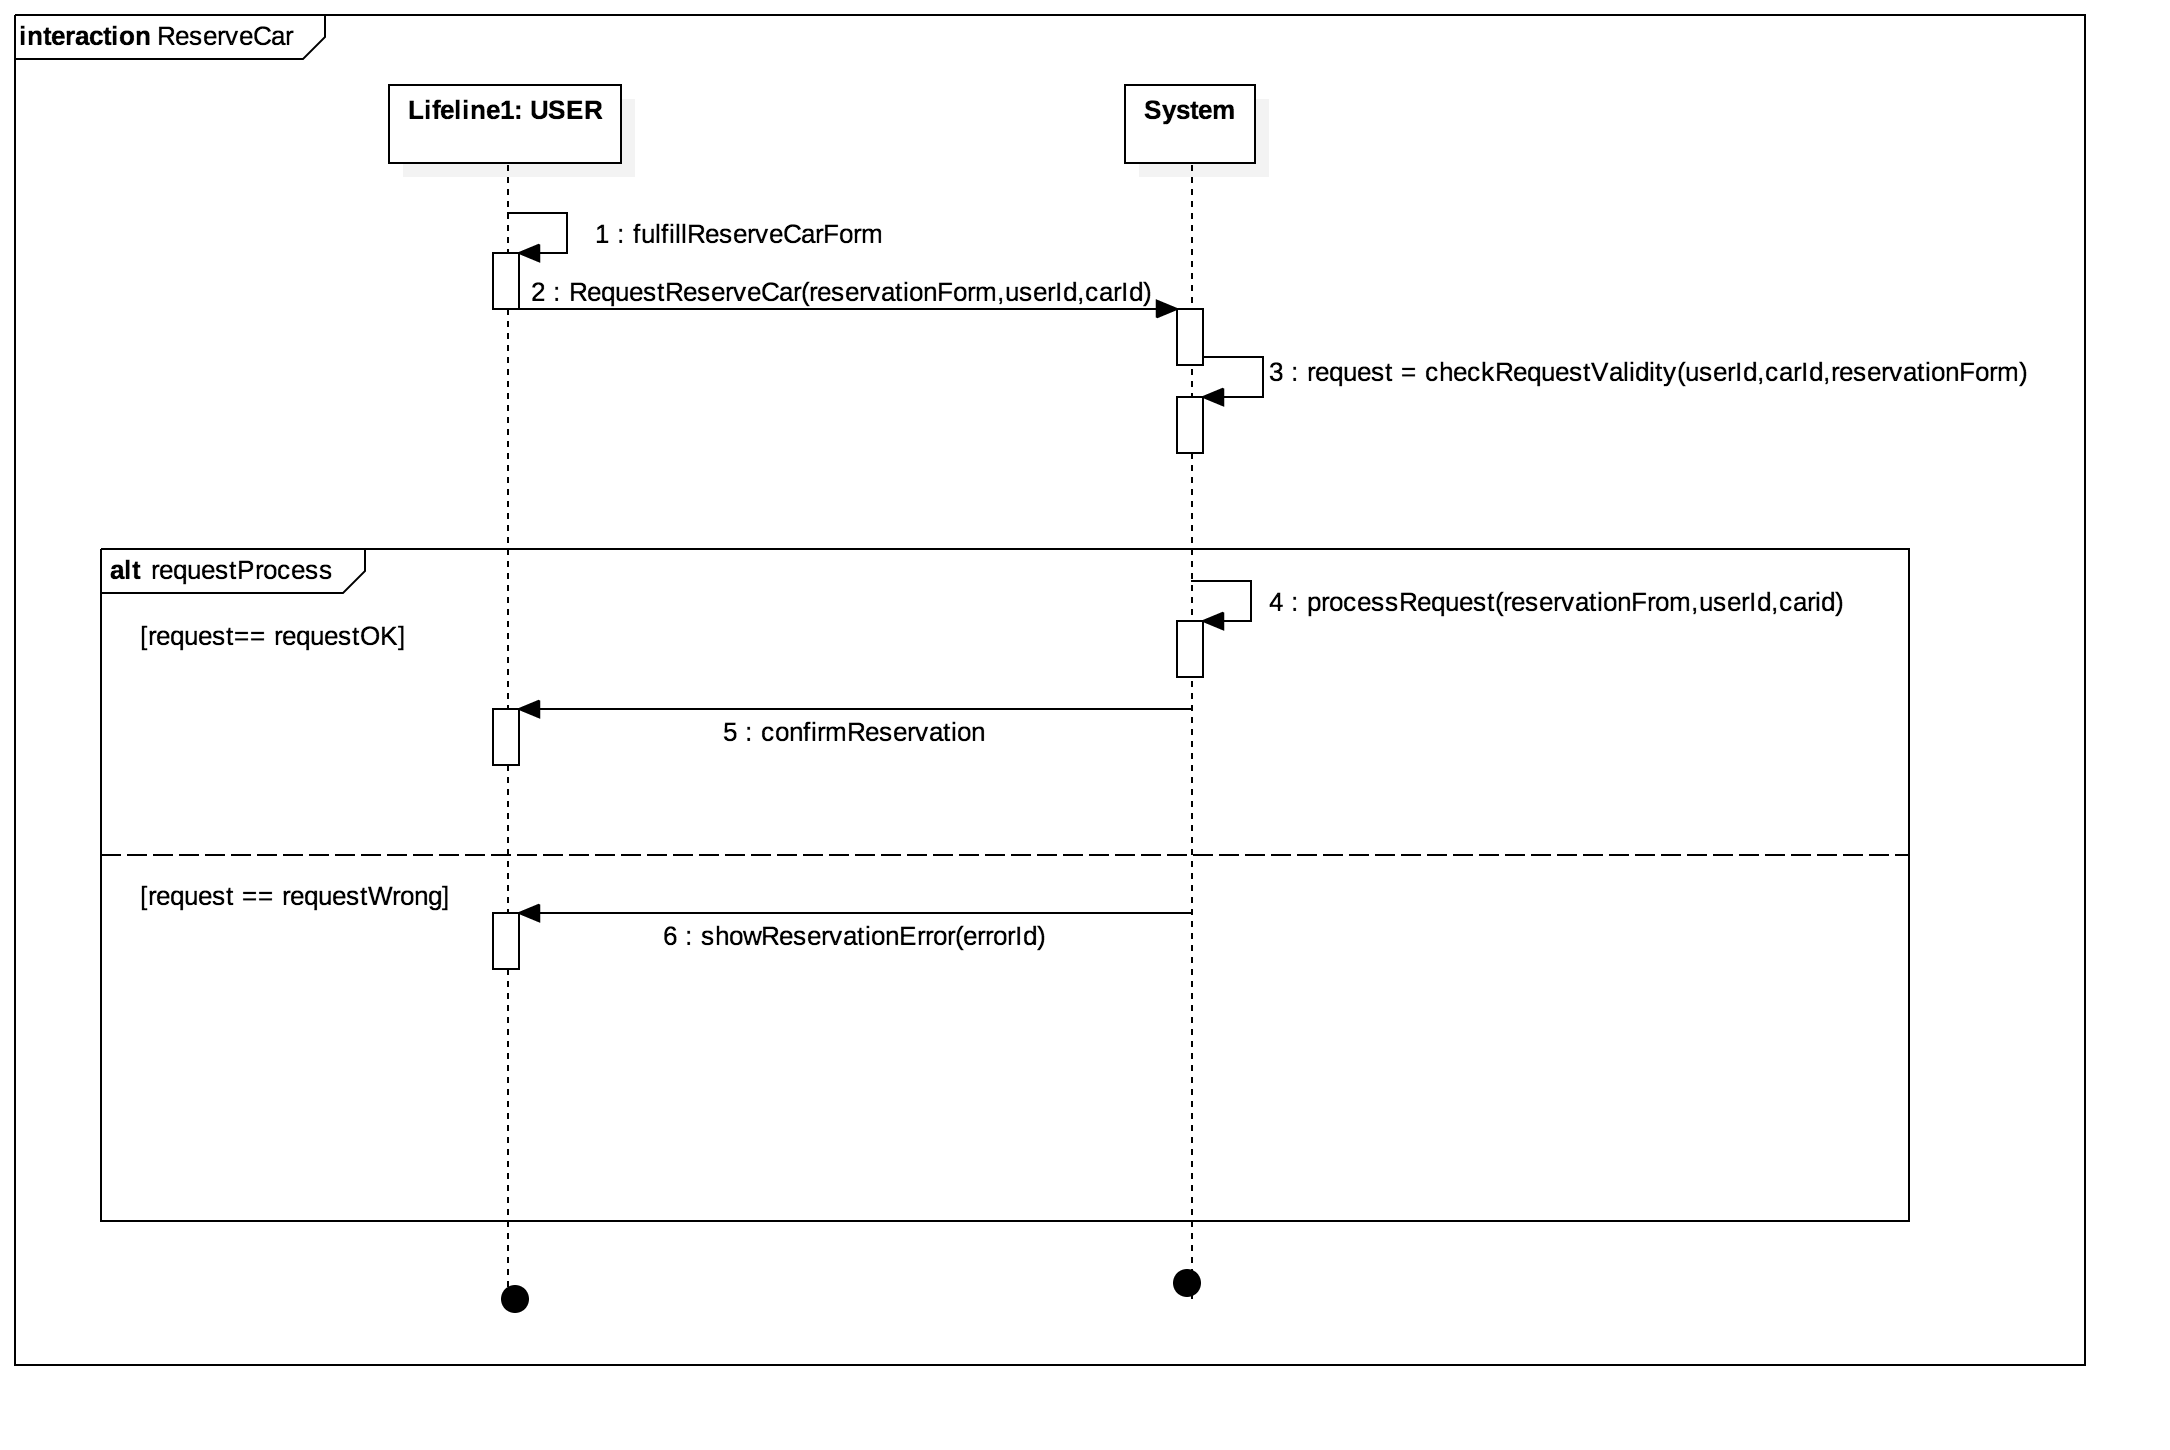
\includegraphics[scale=0.2]{UML/png/Collaboration2__Interaction1__ReserveCar_6}

\caption{Car Reservation}

\end{figure}
\par\end{center}

\subsubsection{Search Cars}

\begin{tabular}{|c|>{\raggedright}p{10cm}|}
\hline 
$\boldsymbol{\mathbf{Name}}$ & Search for Cars\tabularnewline
\hline 
$\mathbf{Actors}$ & USER or GUEST\tabularnewline
\hline 
$\mathbf{Goal}$ & {[}G3.1{]}, {[}G3.2{]} \tabularnewline
\hline 
$\mathbf{EntryConditions}$ & NULL\tabularnewline
\hline 
$\mathbf{EventFlow}$ & \begin{enumerate}
\item User opens the app.
\item User select the search method: search car near his position or near
a selected position.
\item User inserts the needed parameter.
\item The request is sent to the server.
\item Server searches for cars that satisfy requested parameter and sends
them.
\item The App shows the received information.
\end{enumerate}
\tabularnewline
\hline 
$\mathbf{OutputCondition}$ & User or Guest is aware of cars position near to the requested position. \tabularnewline
\hline 
$\mathbf{Exception}$ & No exception.\tabularnewline
\hline 
\end{tabular}\\
\\

\begin{center}
\begin{figure}[H]
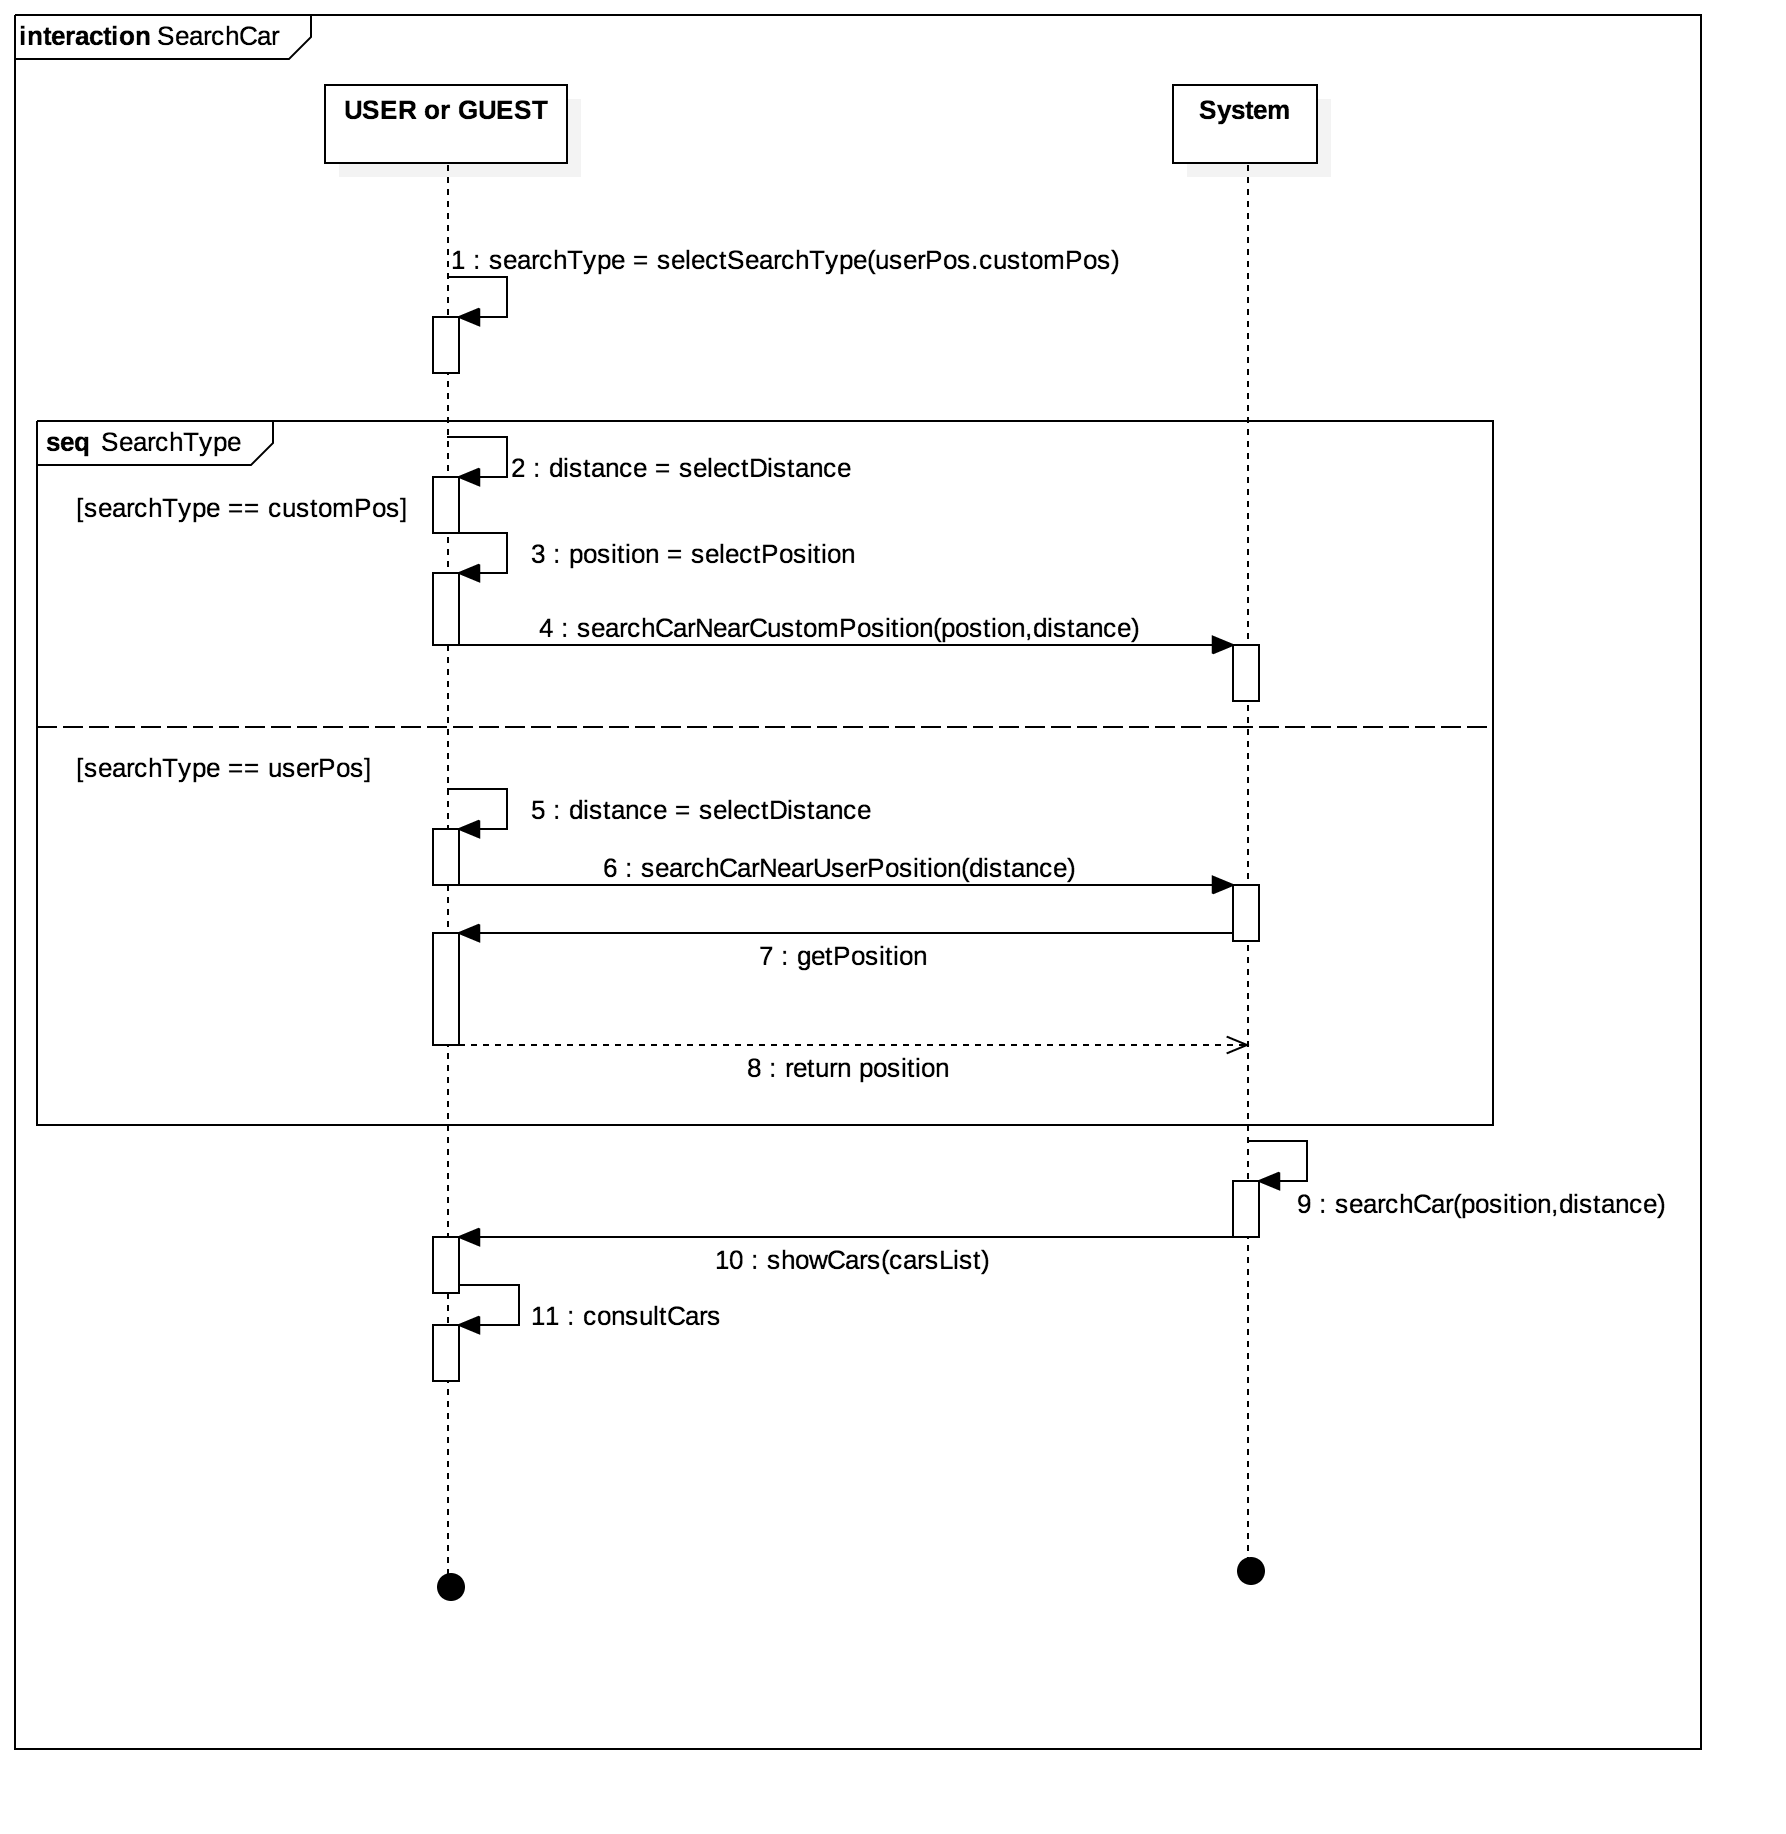
\includegraphics[scale=0.25]{UML/png/Collaboration4__Interaction1__SearchCar_4}

\caption{Search for a car}

\end{figure}
\par\end{center}

\subsubsection{Unlock Car}

\begin{tabular}{|c|>{\raggedright}p{10cm}|}
\hline 
$\boldsymbol{\mathbf{Name}}$ & Unlock Car\tabularnewline
\hline 
$\mathbf{Actors}$ & USER \tabularnewline
\hline 
$\mathbf{Goal}$ & {[}G1.2{]}\tabularnewline
\hline 
$\mathbf{EntryConditions}$ & The user has already reserved a car.\tabularnewline
\hline 
$\mathbf{EventFlow}$ & \begin{enumerate}
\item User opens the app.
\item User make the request, so the client application sends user position
to the server.
\item Server search for the position of the user reserved car.
\item Server check if the distance between car and user is acceptable.
\item If acceptable the car is unlocked.
\end{enumerate}
\tabularnewline
\hline 
$\mathbf{OutputCondition}$ & The user has unlocked is reserved car.\tabularnewline
\hline 
$\mathbf{Exception}$ & \begin{enumerate}
\item The user has not reserved any car.
\item The user is not enoguh close to the car.
\end{enumerate}
In the first case the error is shown to the user.

In the second case the app shows to the user that he have to near
the car if he want to unlock it.\tabularnewline
\hline 
\end{tabular}
\begin{center}
\begin{figure}[H]
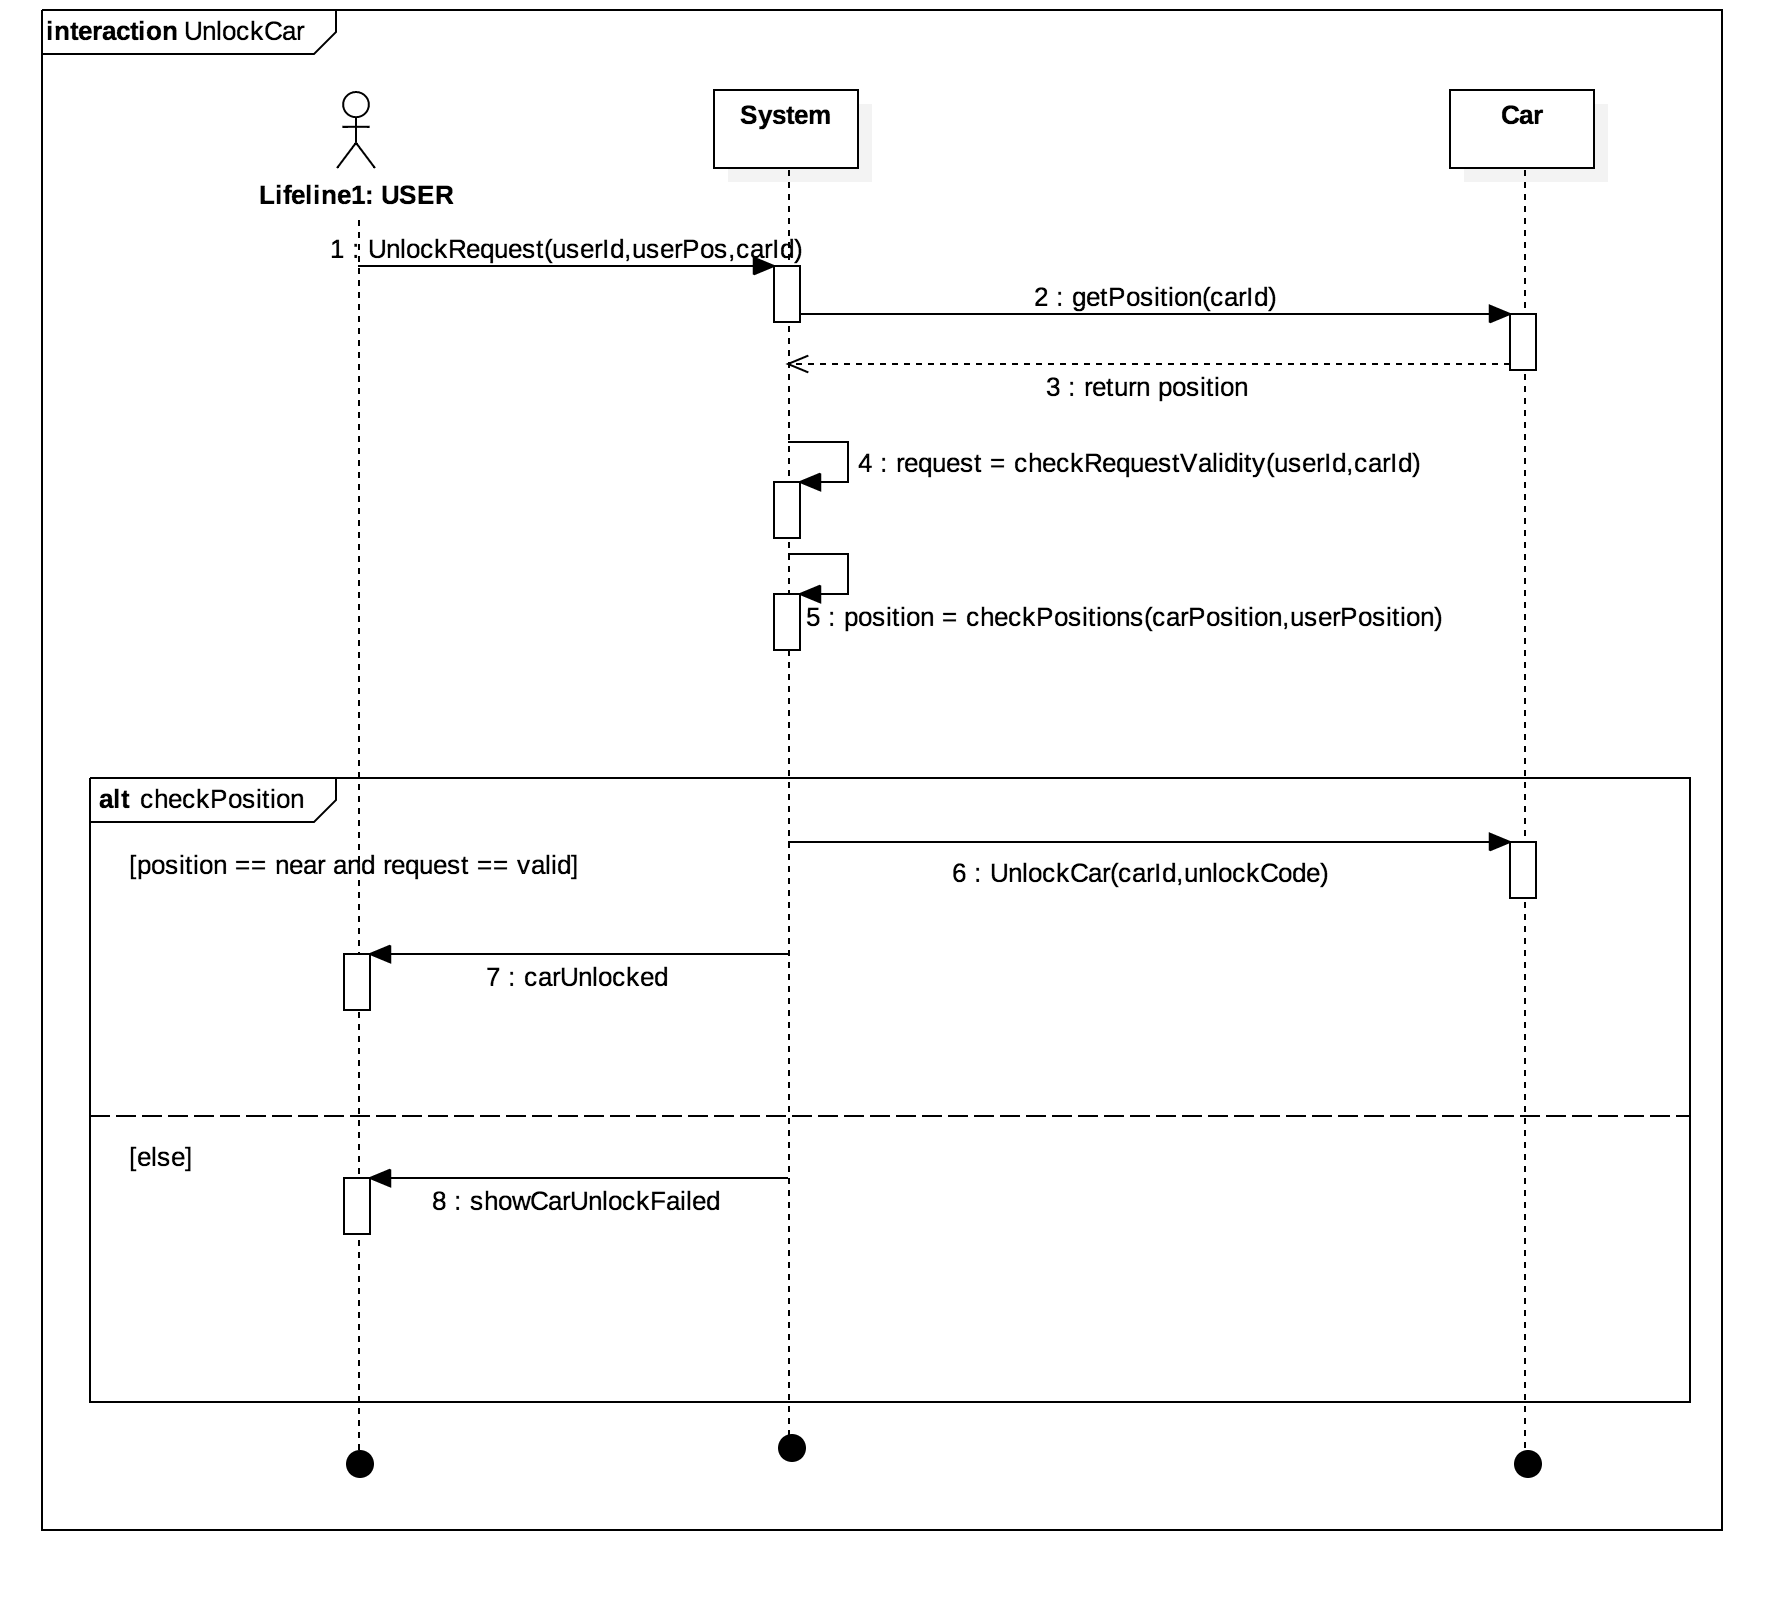
\includegraphics[scale=0.25]{UML/png/Collaboration3__Interaction1__UnlockCar_3}

\caption{Unlock Car}
\end{figure}
\par\end{center}

\subsubsection{Comunicate Damages And Malfucntions}

\begin{tabular}{|c|>{\raggedright}p{10cm}|}
\hline 
$\boldsymbol{\mathbf{Name}}$ & Comunicate Damages And Malfucntions\tabularnewline
\hline 
$\mathbf{Actors}$ & USER \tabularnewline
\hline 
$\mathbf{Goal}$ & {[}G6.2{]}\tabularnewline
\hline 
$\mathbf{EntryConditions}$ & NULL\tabularnewline
\hline 
$\mathbf{EventFlow}$ & \begin{enumerate}
\item User opens the app.
\item User fill the form with description of the damage and identification
of the car.
\item If the form is accepted the server sent an acknowledge to the user
and noificate the operator wich competence area contains the car. 
\end{enumerate}
\tabularnewline
\hline 
$\mathbf{OutputCondition}$ & The user has comunicated a damage to a car or a malfunction.\textbackslash{}\tabularnewline
\hline 
$\mathbf{Exception}$ & \begin{enumerate}
\item The form is not correctly filled.
\end{enumerate}
The request is refused and the user is suggested to check his form.\tabularnewline
\hline 
\end{tabular}
\begin{center}
\begin{figure}[H]
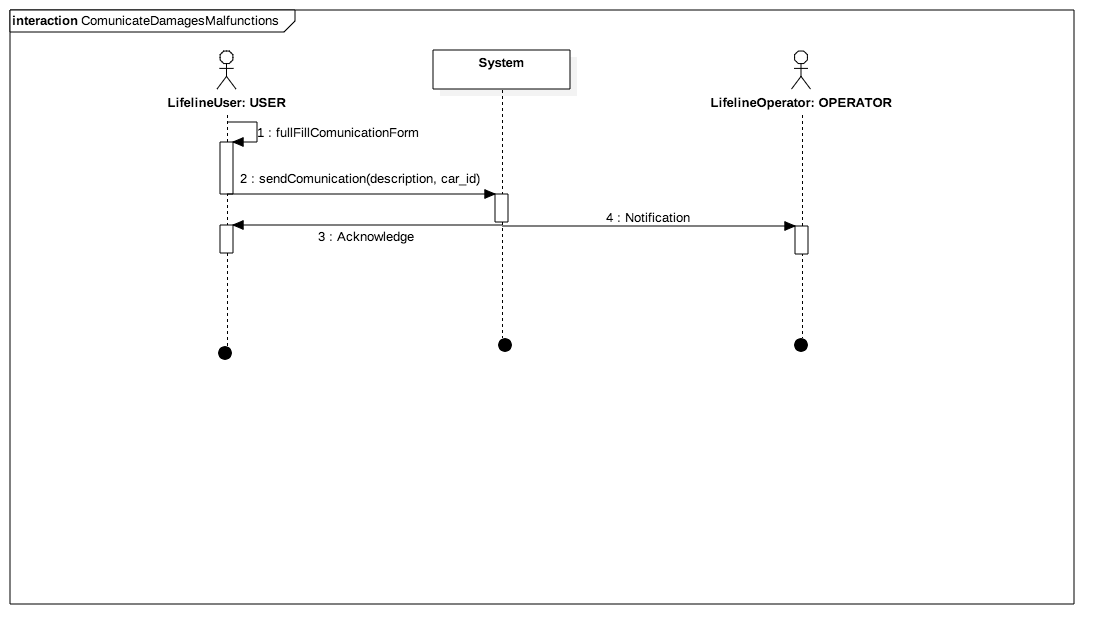
\includegraphics[scale=0.3]{UML/png/ComunicateDamagesMalfunctions}

\caption{Comunicate Damages And Malfucntions}
\end{figure}
\par\end{center}
